
%During routine LSST operations, prompt image data products will be made available 80 hours following camera readout.
%They include raw images, processed single visit images (PVIs), difference images, and template images.
%Access to unvetted PVIs and difference images in the first 6 months of the LSST is still to be decided.


\section{Alert Production in Commissioning and Early Operations}
\label{sec:pp}

The \DPDD{} summarizes the pipelines that will be used during Prompt Processing to produce alerts as well as other prompt data products, including Solar System Processing.
Both Alert Production and Solar System Processing depend on the existence of template images.
During steady-state operations, these templates will be constructed during the annual Data Releases and will be built from the best available subset of images taken.
To enable alert production to proceed during commissioning and early operations, it is necessary build templates incrementally as data become available, as recommended by the study described in \citeds{DMTN-107}.
Because we have a smaller set of input images to choose from and uncertain knowledge about future observations, incremental template generation necessarily must balance the trade-off of earlier template availability against template quality and spatial completeness.
Validation will be required to determine when to build incremental templates to maximize the net throughput of Early Science.
Nevertheless, our goal is to enable Alert Generation to begin over at least a subset of the survey area as soon as the data are scientifically useful.

Scientifically it is important that once a template is constructed for a given region of sky, it is used exclusively until it can be updated in the next Data Release.
Repeated changes to the template make it extremely difficult to construct usable lightcurves for objects from individual difference image sources: transient objects such as supernovae will be contaminated by changing flux levels from the evolving template, and variable objects such as variable stars and AGN will require repeated corrections for different template flux levels as well.

During commissioning templates will be generated incrementally over the maximal sky area supported by the available observations.
By the end of the commissioning period, coadd templates for use in difference imaging will only be available for $\approx$ 10\% of the sky.
Generating templates over a wide area is not an explicit goal of commissioning;  however, where possible, if commissioning observations are agnostic to pointing and filter, we would endeavour to choose a pointing and filter that maximizes building templates to enable early science.

Rubin aims to scale up alert production during commissioning with the aim of beginning routine Alert Production over a progressively increasing fraction of the sky as soon as is feasible following Rubin First Light  (\S~\ref{sec:timeline}).
\citeds{RTN-061} describes the criteria for sending the first Rubin alerts.
Once begun, Alert Production will then proceed continuously into the full LSST survey.
Alerts generated during the early science period may be produced with higher latency, and access to images and the PPDB may not be available during this phase.
During the first phases of Alert Production, alert packets for moving objects might not include the associated historical source records , and parameters such as phase curve slope (G) would be empty until sufficient detections exist to derive them.

Table~\ref{tab:prompt-data-products} lists the various alert and prompt processing data products currently planned at each phase of alert production during commissioning and the first two years of the LSST survey. 
Phase 1 covers the commissioning period and phase 2 covers early survey operations.  
During routine LSST operations, prompt image data products, including  raw images, processed single visit images (PVIs), difference images, and template images, will be made available no earlier than 80 hours following camera readout. 
During the first 6 months of the LSST,  prompt PVIs and difference images may be released with higher latency as Rubin continues to understand data quality and scale up services.


\begin{table}
\centering
\fontsize{6}{10}\selectfont 
\setlength{\tabcolsep}{6pt} % Default value: 6pt
{\renewcommand{\arraystretch}{1.3}
    \begin{tabular}{|p{0.31\linewidth} | p{0.32\linewidth}  | p{0.32\linewidth}|}
    \hline
    \multicolumn{3}{|l|}{{\fontsize{9}{12}\selectfont \color{RubinDarkTeal}\textbf{Rubin Early Science -- Alerts \& Prompt Products Scenario}}}  \\\hline\hline
  

\multirow{1}{*} {}  & 
        \tiny  \makecell{Phase 1: 3 -- 16 weeks post System First Light}  & 
        \tiny   \makecell{Phase 2: 18 -- 17 weeks post System First Light} \\[5pt] \cline{2-3}        
        {\parbox{0.5\linewidth}{\vspace{0.6cm} \textbf{Data Product}}}  &   
        { \makecell{ \textbf{LSSTCam Commissioning }  }}  & 
        {\makecell{\textbf{Year 1 Survey} \\ \textbf{Operations} }} 
         \\[10pt] \cline{2-3} \hline

\textbf{Alerts}     &  Alert volume and latency will improve throughout the commissioning period. Aiming for ``near-live'' brokered Alert stream by the end of LSSTCam Commissioning.  &  
Continued ramp up of the alert stream contingent on the availability of templates.  Alerts expected to reach near full volume and fidelity after DR1.  Alert stream latency in year 1 is 120 seconds. \\  \arrayrulecolor{gray}\hline
%
\textbf{PP Processed Visit Images}     & Commissioning of the PP image differencing and incremental template building. Prompt image release is embargoed during commissioning (\S~\ref{ssec:impact}).  &   Access to processed visit images as prompt products in the first 6 months of the LSST is TBD.      \\  \arrayrulecolor{gray}\hline
\textbf{PP Difference Images}     & Difference imaging will be somewhat limited, since the image template sky coverage will be sparse. Prompt image release is embargoed during commissioning (\S~\ref{ssec:impact}). &     Difference imaging will steadily increase as incremental template building increases the templates available. Access to PP difference images in the first 6 months of LSST is TBD.    \\\hline
%
\textbf{PP Catalogs}    &   Queryable PPDB available at shared risk. &  PPDB available for query. \\ 
 (DIASources, DIAObjects, DIAForcedSources)  & & \\\hline
%
\textbf{PP SSP Catalogs}   &   Measurements of known SSObjects sent to the MPC whenever difference images are available. Searches for new SSObjects performed if appropriately-cadenced data is present. SSP Catalogs likely unavailable for query in the PPDB. &   Standard SSP Daily Data Products produced from difference images as they are available and reported to the MPC. SSP catalogs available for query in the PPDB.  \\  \hline

\arrayrulecolor{black}\hline
\end{tabular}}
\caption{Summary of Prompt data products expected during commissioning and year 1 of survey observations..}
\label{tab:prompt-data-products}
\end{table}

%\begin{table}[ht]
%\centering
%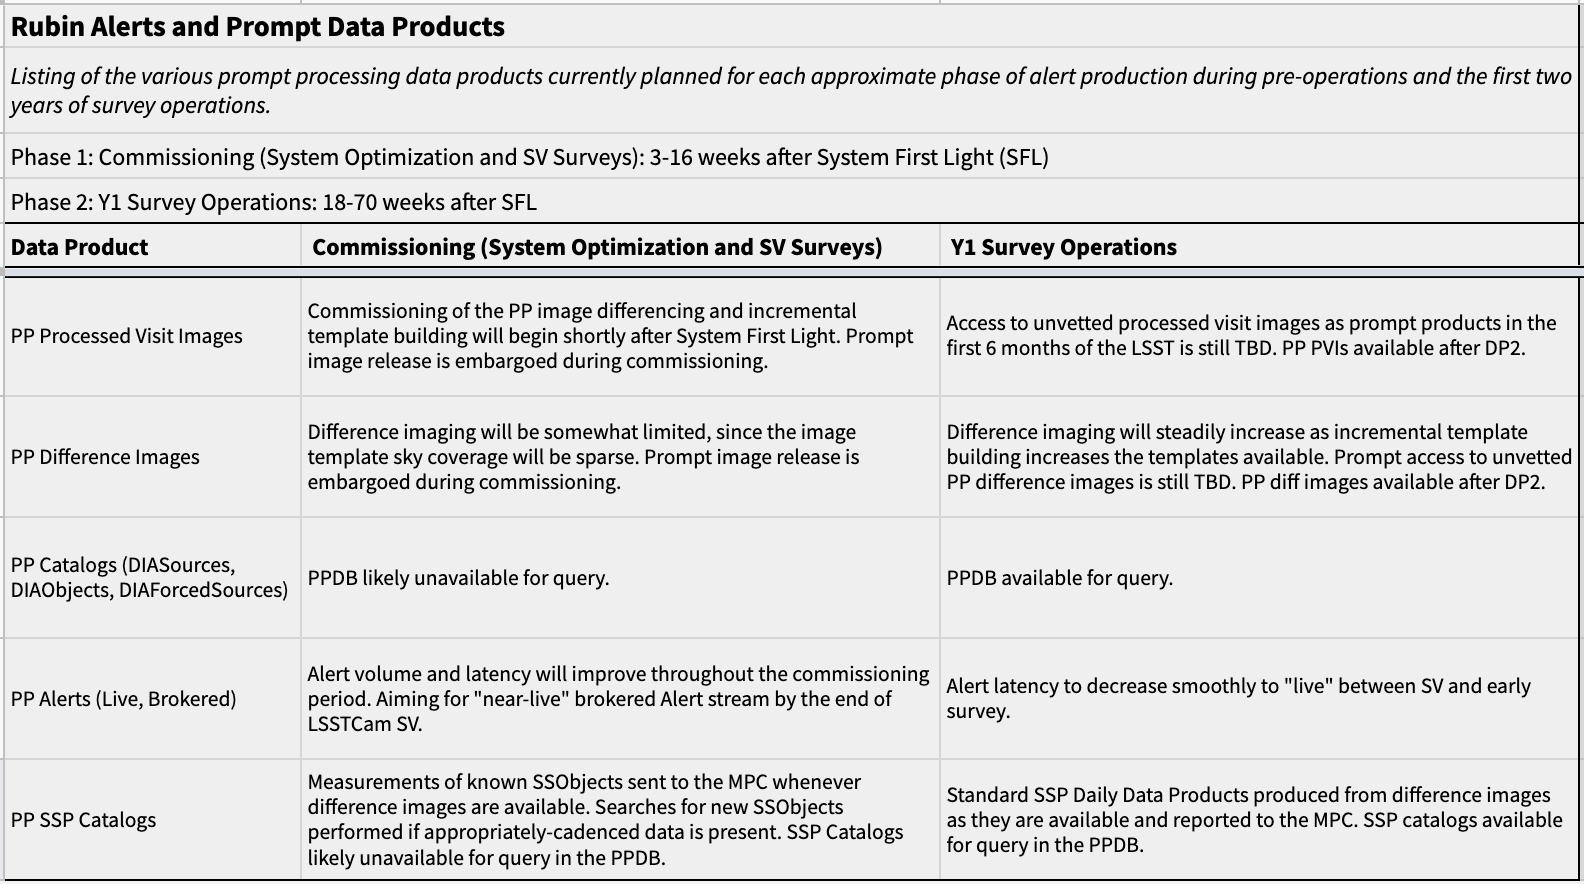
\includegraphics[width=0.9\linewidth]{figures/Prompt-products}
%\caption{Summary of prompt data products expected during commissioning and year 1 survey observations.}
%\label{tab:prompt-data-products}
%\end{table}

